\documentclass{beamer}
\usepackage{xspace}
\usepackage{graphicx}
\usepackage{epsfig}
%\usepackage{figlatex}
\usepackage{verbatim}
%\usepackage{listings}

\usepackage{subfigure}

%\usepackage{algorithm}
%\usepackage[noend]{algpseudocode}


\usepackage[ruled,vlined]{algorithm2e}

\usepackage{float}

\usetheme{Madrid}
 \setbeamertemplate{navigation symbols}{}
 \setbeamercovered{transparent}

\newcommand{\card}[1]{\ensuremath{|#1|}}
\newcommand{\union}{\ensuremath{\cup}}

\newcommand{\ceil}[1]{\left\lceil#1\right\rceil}
\newcommand{\floor}[1]{\lfloor#1\rfloor}
\newcommand{\todo}[1]{{\bf TODO: #1}}

\usealerttemplate{\color{red}\bf}{}

\graphicspath{{fig/}}

\newcommand{\MIC}{Intel MIC\xspace}

\title[RBF-FD on \MIC]{Acceleration of Derivative Calculations with
  Application to Radial Basis Function ­ Finite-Differences on the
  Intel MIC Architecture}

\date{ICS 2014}

\author[Erik Saule]{Gordon Erlebacher, {\bf Erik Saule}, Natasha Flyer, Evan
  Bollig}
 
\institute[UNCC]{Florida State University\\{\bf University of North Carolina at Charlotte}\\UCAR\\University of Minnesota}

\begin{document}

\maketitle

\begin{frame}
  \frametitle{Outline}
  \tableofcontents[hidesubsection,hidesubsubsection]
\end{frame}

\section{Radial Basis Function - Finite Difference}

\AtBeginSection[]
{
  \begin{frame}<beamer>
    \frametitle{Outline}
    \tableofcontents[currentsection]
  \end{frame}
}

\begin{frame}[fragile]
  \frametitle{Derivative as (sparse) linear algebra operators}

  \begin{columns}
    \column{.5\linewidth}
    \begin{block}{2nd derivative, 1D}

      \includegraphics[width=\linewidth]{slides-figures/1d.pdf}

      $$u''_i = \frac{u_{i+1}-2u_i+u_{i-1}}{h^2}$$
      \scalebox{.8}{$A = \begin{pmatrix}
        \dots & \dots & \dots & \dots & \dots & \dots & \dots \\
        \dots & 1 & -2 & 1 & 0 & 0 & \dots  \\
        \dots & 0 & 1 & -2 & 1 & 0 & \dots \\
        \dots & 0 & 0 & 1 & -2 & 1 & \dots  \\
        \dots & \dots & \dots & \dots & \dots & \dots & \dots
      \end{pmatrix}$}
      $$u'' = Au$$
    \end{block}
    
    \column{.49\linewidth}
    \begin{block}{2nd derivative, 2D}
      \begin{center}
        \includegraphics[width=.6\linewidth]{slides-figures/2d.pdf}
      \end{center}
      
        $L_{i,j} = \bigtriangledown^2 u_{i,j} = \frac{1}{h^2} (u_{i+1,j}  +u_{i-1,j}$
        
        $~~~~~~~~~~~~~~~~+u_{i,j-1}+u_{i,j+1}-4u_i)$
    \end{block}    
    
  \end{columns}
\end{frame}

\begin{frame}[fragile]
  \frametitle{Radial Basis Function}
  \begin{columns}
    \column{.45\linewidth}

    \begin{block}{RBF}
      \includegraphics[width=\linewidth]{slides-figures/rbf.pdf}
      
      \begin{itemize}
      \item Radial symmetry.
      \item RBFs approximate a function $f$ sampled at $N$ distinct locations $$f(\vec{r}) = \sum_i w_i \phi(||\vec{r}-\vec{r_i}||)$$ 
      \end{itemize}
    \end{block}
    
    \column{.45\linewidth}
    \begin{block}{The RBF-FD method}
      \includegraphics[width=.8\linewidth]{slides-figures/ICS-figures/RBFStencil_n32_a}
      
      Derivative operators of an RBF are approximated using the $n=32$
      closest sampling points on a sphere of $N=1024$ points.

      The DM has exactly $n$ non-zeros per row.
    \end{block}
    
  \end{columns}
\end{frame}


\begin{frame}
  \frametitle{Computing derivatives. One at a time?}
  
  \begin{block}{Shallow waters equations}
    
    \begin{eqnarray}
      \dfrac{\partial u}{\partial t} &=& - \left( u\dfrac{\partial u}{\partial x} + v\dfrac{\partial u}{\partial y} + w\dfrac{\partial u}{\partial z} + f(yw - zv) + g\dfrac{\partial h}{\partial x} \right) 
      \nonumber \\
      \dfrac{\partial v}{\partial t} &=& - \left( u\dfrac{\partial v}{\partial x} + v\dfrac{\partial v}{\partial y} + w\dfrac{\partial v}{\partial z} + f(zu - xw) + g\dfrac{\partial h}{\partial y} \right)
      \nonumber\\
      \dfrac{\partial w}{\partial t} &=& - \left( u\dfrac{\partial w}{\partial x} + v\dfrac{\partial w}{\partial y} + w\dfrac{\partial w}{\partial z} + f(xv - yu) + g\dfrac{\partial h}{\partial z} \right) 
      \nonumber\\
      \frac{\partial h}{\partial t} &=& -\left(\dfrac{\partial (uh)}{\partial x} + \dfrac{\partial (vh)}{\partial y} + h\dfrac{\partial (wh)}{\partial z}\right)  \nonumber
    \end{eqnarray}
    $u,v,w$ velocity. $h$ geopotential height.
  \end{block}
  
  One at a time? $\dfrac{\partial u}{\partial x}$, then $\dfrac{\partial v}{\partial y}$

  \only<2>{\vspace{-19em}\hspace{-1em}\begin{minipage}{.95\linewidth}
      \colorbox{white}{
        \includegraphics[width=\linewidth]{slides-figures/PPAM-figures/all_compare_spmv.pdf}
        \tiny PPAM 2013
      }
    \end{minipage}}
  
\end{frame}
  

\begin{frame}
  \frametitle{Compute all the simple derivatives at once}

\only<1-2>{  \begin{block}{Shallow waters equations}
    \begin{eqnarray}
      \dfrac{\partial u}{\partial t} &=& - \left( u\dfrac{ \textcolor{blue}{\partial}  u}{\textcolor{blue}{\partial x}} + v\dfrac{\textcolor{red}{\partial} u}{\textcolor{red}{\partial y}} + w\dfrac{\textcolor{green}{\partial} u}{\textcolor{green}{\partial z}} + f(yw - zv) + g\dfrac{\textcolor{blue}{\partial} h}{\textcolor{blue}{\partial x}} \right) 
      \nonumber \\
      \dfrac{\partial v}{\partial t} &=& - \left( u\dfrac{ \textcolor{blue}{\partial} v}{\textcolor{blue}{\partial x}} + v\dfrac{\textcolor{red}{\partial} v}{\textcolor{red}{\partial y}} + w\dfrac{\textcolor{green}{\partial} v}{\textcolor{green}{\partial z}} + f(zu - xw) + g\dfrac{\textcolor{red}{\partial} h}{\textcolor{red}{\partial} y} \right)
      \nonumber \\
      \dfrac{\partial w}{\partial t} &=& - \left( u\dfrac{\textcolor{blue}{\partial} w}{\textcolor{blue}{\partial x}} + v\dfrac{\textcolor{red}{\partial} w}{\textcolor{red}{\partial y}} + w\dfrac{\textcolor{green}{\partial} w}{\textcolor{green}{\partial z}} + f(xv - yu) + g\dfrac{\textcolor{green}{\partial} h}{\textcolor{green}{\partial z}} \right) 
      \nonumber\\
      \frac{\partial h}{\partial t} &=& -\left(\dfrac{\partial (uh)}{\partial x} + \dfrac{\partial (vh)}{\partial y} + h\dfrac{\partial (wh)}{\partial z}\right)  \nonumber
    \end{eqnarray}
  \end{block}}
  
\pause

  \begin{block}{Idea}
    \scriptsize
    \begin{equation}
      \left( \begin{array}{cccc}
          \underline{u}_x     & \underline{v}_x     & \underline{w}_x     & \underline{h}_x \\
          \underline{u}_y     & \underline{v}_y     & \underline{w}_y     & \underline{h}_y \\
          \underline{u}_z     & \underline{v}_z     & \underline{w}_z     & \underline{h}_z \\
          \underline{u}_{hyp} & \underline{v}_{hyp} & \underline{w}_{hyp} & \underline{h}_{hyp}
        \end{array} \right)
      = \left(
        \begin{array}{c}
          \textcolor{blue}{D_{x}}\\ \textcolor{red}{D_{y}}\\ \textcolor{green}{D_{z}}\\ D_{hyp}
        \end{array}\right)
      \times \left(\underline{u} \,\, \underline{v} \,\, \underline{w} \,\, \underline{h} \,\,\right) \nonumber
      \vspace{-1ex}
    \end{equation}
  \end{block}  
  
\pause
    
  \begin{block}{Why would it work}
    All the derivative matrices have the same sparsity pattern.

    In other words, the non zeros are at the same positions in the
    matrix, only the non-zero values change.

    Benefits:
    \begin{itemize}
    \item Matrix compression: 1 column ID, 4 non-zero values. (gain: 38\%)
    \item Vector reusage.
    \end{itemize}
  \end{block}
\end{frame}

\section{Performance Prediction}


\begin{frame}
  \frametitle{Is there hope in this technique? Let's model it.}

  \begin{columns}
    \column{.4\linewidth}
    \scalebox{.55}{
      \begin{tabular}{|c|l|}
        % \hline
        % & & \\
        \hline
        $b_i$ & number of bytes per index \\
        $b_x$ & number of bytes per value \\
        $n_z$ & number of nonzeros per row of $A$ \\
        $n_r$ & number of column/rows of $A$ \\
        $n_c$ & total number of nonzeros\\
        $n_v$ & number of {\tt x} vectors \\
        $n_m$ & number of matrices \\
        $s_M$ & size of the $n_m$ matrices in bytes\\
        $s_x$ & size of the $n_v$ {\tt x} vectors in bytes\\
        $s_y$ & size of the $n_v n_m$ {\tt y} vectors in bytes\\
        \hline
        $cl$    & size of a cache line in bytes\\
        $b_{wT}$ & number of bytes written to memory  \\
        $b_{rT}$ & minimum number of bytes read from memory  \\
        $b_T$   & minimum number of bytes transferred \\
        $B_{rT}$ & maximum number of bytes read from memory \\
        $B_T$   & maximum number of bytes transferred \\
        $O$     & number of floating point operations \\
        $I_b$   & maximum computational intensity\\
        $I_w$   & minimum computational intensity\\        
        \hline
      \end{tabular}
    }
    \column{.6\linewidth}

    Size of the input vector:\\$s_x = n_v b_x n_r$

    Size of the matrix:\\$s_M = n_c (b_i + b_x n_m) = n_r n_z (b_i + b_x n_m)$

    Size of the write (output vector):\\$b_{wT} = s_y = n_v n_m b_x n_r$

    Data Read (best case):\\$b_{rT} = s_M + s_x$
    
    Data Read (worst case):\\$B_{rT} = s_M + n_c cl \ceil{\frac{n_vb_x}{cl}}$

    Number of floating point operations:\\$O = 2 n_v n_m n_c = 2 n_v n_m n_z n_r$
  \end{columns}

  \begin{center}
    Intensity (Best case):\\
    $I_b = \frac{O}{b_T+ b_{wT}} = \frac{2 n_v n_m}{ (b_i + b_x n_m) + n_v n_m b_x n_z^{-1} + n_v b_x n_z^{-1} }$
    
    Intensity (Worst case):\\
    $I_w = \frac{O}{B_T+ b_{wT}} = \frac{2 n_v n_m}{(b_i+b_x n_m) + n_v n_m b_x n_z^{-1} + cl \ceil{\frac{n_vb_x}{cl}} }$
  \end{center}
\end{frame}

\begin{frame}
  \frametitle{Ok... So will it work? Flop to byte ratio}

  \begin{columns}
\only<1>{    \column{.49\linewidth}
    \includegraphics[width=\linewidth]{slides-figures/ICS-figures/flops_to_bytes_best-crop.pdf}

    \begin{center}
      Best case\\~
    \end{center}
}
    \column{.49\linewidth}
    \includegraphics[width=\linewidth]{slides-figures/ICS-figures/flops_to_bytes_worst-crop.pdf}
    \begin{center}
      Worst case\\~
    \end{center}

\only<2>{
    \column{.49\linewidth}
    \includegraphics[width=\linewidth]{slides-figures/ICS-figures/flops_to_bytes_no_cache-crop.pdf}
    \begin{center}
      Worst case \\no cacheline
    \end{center}
}
  \end{columns}

%  \tiny Also, taking cacheline into account makes a large difference (see paper for details).
\end{frame}

\begin{frame}
  \frametitle{In terms of flops? (Assuming memory bandwidth bound)}

  \includegraphics[width=.9\linewidth]{slides-figures/ICS-figures/gflops_peak.pdf}

\end{frame}


\section{Implementation on Xeon Phi (4 vectors, 4 matrices, Single Precision)}

% \begin{frame}
%   \frametitle{Intel MIC: Overall Architecture}
%   \begin{columns}
%     \column{18em}    
%     \includegraphics[width=18em]{slides-figures/MIC-overview.pdf}
%     \column{17em}
    
%     \begin{itemize}
%       \item 8 memory controllers
%         \begin{itemize}
%           \item GDDR5
%           \item 2 channels (32-bit)
%           \item 5.5GT/s
%           \item 352GB/s aggregated peak
%             \begin{itemize}
%               \item about same as a K40 
%               \item but you typically get half
%             \end{itemize}
%         \end{itemize}
%       \item 50+ cores
%         \begin{itemize}
%           \item 32KB of L1 cache
%           \item 512KB of L2 cache
%           \item LRU
%           \item 8-way associative
%         \end{itemize}
%       \item 1 PCI-e controller
%         \begin{itemize}
%           \item to the host (2GB/s guaranteed to memory)
%         \end{itemize}
%     \end{itemize}
%   \end{columns}

% \end{frame}

% \begin{frame}
%   \frametitle{Core architecture}
%   \begin{columns}
%     \column{20em}
%     \includegraphics[width=20em,height=20em]{slides-figures/MIC-core.png}%from intelsdg  
%     \column{12em}
%     \begin{itemize}
%       \small
%     \item Clocked at 1Ghz
%     \item 64-bit
%     \item 4 hardware threads
%       \begin{itemize}
%         \footnotesize
%         \item no context switching
%         \item no 2 instructions for the same thread
%       \end{itemize}
%     \item A vectorial unit
%       \begin{itemize}
%         \footnotesize
%         \item 512-bit registers
%         \item 16 SP floats
%         \item 8 DP floats
%         \item support FMA
%       \end{itemize}
%     \item Two instruction pipes:
%       \begin{itemize}
%         \footnotesize
%         \item 2 ALU ops
%         \item ALU + MEM ops
%         \item ALU + VFP ops
%         \item VFP + MEM ops
%       \end{itemize}
%     \item In-order execution
%     \end{itemize}
%   \end{columns}
% \end{frame}

\begin{frame}
  \frametitle{Summary of \MIC}

  \begin{block}{Key points of Xeon Phi SE10P}
    \begin{itemize}
    \item Accelerator card (soon main processor with Knights Landing) 
    \item Large memory bandwidth (peak: 220GB/s)
    \item 61 cores with mandatory use of hardware threading
    \item Mandatory use of 512-bit wide SIMD registers: 
      \begin{itemize} 
      \item FMA: up to 2x16 SP Flop/c (2x8 DP Flop/c)
      \item otherwise: up to 16 SP Flop/c (8 DP Flop/c)
      \end{itemize}
    \item On a 61-core configuration at 1.05Ghz:
      \begin{itemize} 
      \item FMA: 2x16x61x1.05Ghz = 2.048 TFlop/s SP (1.024TFlop/s DP)
      \item otherwise: 16x61x1.05Ghz = 1.024 GFlop/s SP (512GFlop/s DP)
      \end{itemize}
    \end{itemize}
  \end{block}

  Lots of bandwidth? Fused Multiply Add? Large vector registers?

  Sounds like the perfect system for scientific computing!
\end{frame}


\begin{frame}
  \frametitle{Observations on the 4 vectors, 4 matrices case}

  \begin{itemize}
  \item We aim at over 200Gflop/s in single precision.
  \item Peak of Xeon Phi is 2TFlop/s.
  \item We want 10\% of peak performance.
  \item One instruction in ten must be a Fused Multiply Add.
  \item The kernel must be fairly instruction-efficient.
  \end{itemize}
\end{frame}

\begin{frame}
  \frametitle{Vectorial Unit (SIMD) : Rearranging}

  \begin{columns}
    \column{.45\linewidth}

    \hspace*{-.1\linewidth}\includegraphics[width=1.2\linewidth]{slides-figures/vect-swizzling.png}%from intelsdg
    
    \column{.45\linewidth}
    
    Registers are organized in 4 lanes.

    \begin{block}{Permutation}
      Permutation instructions allow to reorder lanes according to
      given patterns.
    \end{block}
    
    \begin{block}{Swizzling}
      Almost all instructions support recombining elements within a
      lane. As it is part of the instruction, swizzling comes with no
      throughput penalty (but certainly a high latency). These also
      typically follow a given set of patterns.
    \end{block}
  \end{columns}
\end{frame}

\begin{frame}
  \frametitle{Vectorial Unit (SIMD) : smarter loads}
  
  \begin{columns}
    \column{.45\linewidth}

    \begin{block}{Gather}
      Allows to load data from memory at arbitrary offsets. Takes one
      cycle per cache line accessed.
    \end{block}
    \includegraphics[width=\linewidth]{slides-figures/gather.pdf}

    \column{.45\linewidth}
  
    \begin{block}{Unpack}
      Allows to load packed data from memory using a bit mask write.
    \end{block}
     
    \includegraphics[width=\linewidth]{slides-figures/unpack.pdf}
 
  \end{columns}
\end{frame}

\begin{frame}
  \frametitle{How to do it? (4 vectors, 4 matrices)}
  
  \begin{figure}
    \centering
    \hspace*{-1em}\scalebox{.95}{
      \subfigure[Source code]{\includegraphics[clip=true,trim=4.5cm 11cm 4cm 4.2cm,width=.6\linewidth]{slides-figures/ICS-figures/code.pdf}}%
      \subfigure[Content of the vector registers.]{\hspace{-0.07\linewidth}\includegraphics[width=.55\linewidth]{slides-figures/ICS-figures/code-annote.pdf}}
    }
  \end{figure}  
\end{frame}

\section{Experiments}

\begin{frame}
  \frametitle{Results : Extreme cases}
  \begin{columns}
    \column{.4\linewidth}
    
    \begin{block}{Supercompact}
      \centering
      \includegraphics[width=.6\linewidth]{slides-figures/ICS-figures/supercompact_matrix-crop.png}
    \end{block}
  
    \begin{block}{Random}
      \centering
      \includegraphics[width=.6\linewidth]{slides-figures/ICS-figures/random_matrix-crop.png}
    \end{block}
    
    \column{.6\linewidth}
    \includegraphics[width=\linewidth]{slides-figures/ICS-figures/random_supercompact.pdf}
  \end{columns}
\end{frame}

\begin{frame}
  \frametitle{Results : Real cases}
  \begin{columns}
    \column{.4\linewidth}
    \begin{block}{Compact}
      \centering
      \includegraphics[width=.6\linewidth]{slides-figures/ICS-figures/compact_matrix-crop.png}
    \end{block}
  
    \begin{block}{RBF-FD}
      \centering
      \includegraphics[width=.6\linewidth]{slides-figures/ICS-figures/kd-tree-3d-rcm-crop.png}
    \end{block}
    
    \column{.6\linewidth}
    \includegraphics[width=\linewidth]{slides-figures/ICS-figures/rbf_compact.pdf}
  \end{columns}
\end{frame}

\begin{frame}
  \frametitle{Does it help?}
  \begin{center}
    \includegraphics[width=.7\linewidth]{slides-figures/ICS-figures/mic_performance_nb_threads.pdf}
  \end{center}
  
  Performance of $y=Ax$ for a RBF derivative stencil of a $96^3$ 3D
  grid. Shown: The peaks of common methods
\end{frame}


\section{Conclusion}

\begin{frame}
  \frametitle{Conclusion}
  
  \begin{block}{Conclusion}
    \begin{itemize}
    \item RBF-FD needs to compute different derivative of multiple functions.
    \item The different derivatives have the same sparsity structure.
    \item Idea: perform all the derivatives simultaneously
    \item The flop-to-byte ratio increases significantly
    \item Vector reordering operations of Xeon Phi enables efficient execution
    \item Performs efficiently: 
      \begin{itemize}
      \item 3.5 times faster than peak of traditional SpMV  
      \item faster than peak of SpMM (v=4)
      \end{itemize}
    \end{itemize}
  \end{block}

  \begin{block}{Future Works}
    \begin{itemize}
    \item More than 1 Xeon Phi?
    \item More than 1 node?
    \item Perform a complete simulation.
    \item GPU?
    \end{itemize}
  \end{block}
\end{frame}

\begin{frame}
  \frametitle{Thank you}

  \begin{block}{Other related works}
    \begin{itemize}
    \item Scalability of graph algorithms on Intel MIC. (MTAAP 2012)
    \item Sparse Matrix Vector Multiplication on Xeon Phi. (PPAM 2013)
    \item Vectorization of Graph Centrality on Xeon Phi. (MTAAP 2014)
    \end{itemize}
  \end{block}
  
  \begin{block}{More information}
    Contact : esaule@uncc.edu

    Visit: \url{http://webpages.uncc.edu/~esaule}
  \end{block}
\end{frame}

\bibliographystyle{alpha}
\bibliography{slides}

\end{document}
